\subsection{Variable Neighborhood Search}
Variable Neighborhood Search is a optimization algorithm that combines local search with a neighborhood change strategy. The algorithm is made up of three main components:
\begin{itemize}
    \item Shaking: generates a new solution in the neighborhood of the current solution.
    \item Local Search: improves the solution generated by the shaking step. This is done by applying either first-improvement or best-improvement.
    \item Move or Not: if the solution generated by the local search is better than the current solution, the current solution is replaced by the new solution and the size of the neighborhood is reset to $k_{min}$. Otherwise, the size of the neighborhood is increased.
\end{itemize}

In our example we want to solve the KnapSack-01 problem and we thus the neighborhood structure $N_k$ is defined as the set of all solution that can be obtained by switching $k$ bits in the current solution. Thus it's obvious that the performance of the algorithm is highly dependent on the maximum number of bits that can be switched \ref{tab:neighborhood}. Obviously the quality of the solution achieved is also dependent on the stochastic component of the algorithm.
\begin{table}[H]
    \centering
    \begin{tabular}{c||c |c}
        k  & quantity & capacity \\ \hline
        2  & 8        & 6        \\
        5  & 13       & 8        \\
        7  & 13       & 9        \\
        10 & 15       & 9        \\
    \end{tabular}
    \caption{Different neighborhood structures}
    \label{tab:neighborhood}
\end{table}

On the other hand if we have a diverse enough neighborhood structure, the initial point is not as important as the algorithm will be able to explore the search space anyway \ref{tab:start}.
\begin{table}[H]
    \centering
    \begin{tabular}{c||c |c}
        starting point                 & quantity & capacity \\ \hline
        (1, 0, 0, 1, 0, 1, 0, 1, 0, 1) & 15       & 10       \\
        (0, 1, 0, 1, 1, 1, 0, 1, 0, 0) & 14       & 10       \\
        (1, 1, 1, 1, 1, 1, 1, 1, 1, 1) & 14       & 10       \\
        (0, 0, 0, 0, 0, 0, 0, 0, 0, 0) & 16       & 10       \\
    \end{tabular}
    \caption{Different starting points}
    \label{tab:start}
\end{table}

The other important choice that can be made is the choice of the local search algorithm. Obviously, best-improvement yiels better results than first-improvement, but it is also more expensive. In our case, the problem is small enough that there isn't a big difference between the two \ref{fig:vns}.
\begin{figure}[H]
    \begin{subfigure}{0.5\textwidth}
        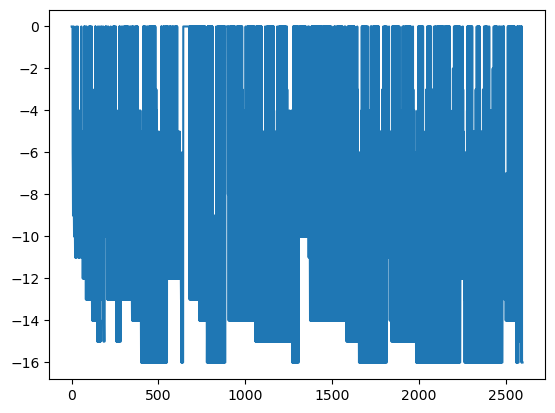
\includegraphics[width=\textwidth]{lab4/imgs/vns_best.png}
        \caption{Best-improvement}
    \end{subfigure}
    \begin{subfigure}{0.5\textwidth}
        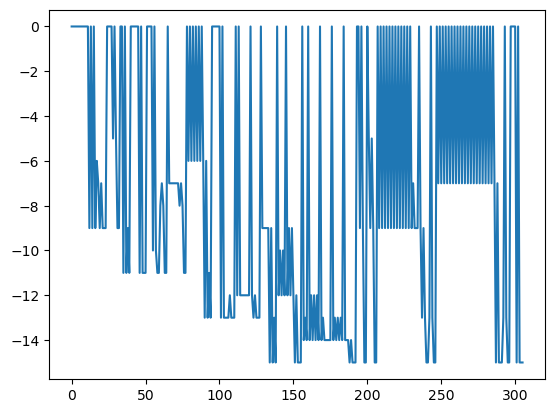
\includegraphics[width=\textwidth]{lab4/imgs/vns_first.png}
        \caption{First-improvement}
    \end{subfigure}
    \caption{VNS with different local search algorithms}
    \label{fig:vns}
\end{figure}


\subsection{Reduced Variable Neighborhood Search}
Reduced Variable Neighborhood Search is a variant of the VNS algorithm that skips the most expensive step of VNS which is the local search.

Similarly to VNS, if the neighborhood structure is diverse enough the starting is not very important \ref{tab:rvns-start} but if the neighborhood is limited then it becomes very important. For example in table \ref{tab:rvns-neigh} we can see that for $k=2$ the algorithm was unable to find a valid solution.
\begin{table}[H]
    \centering
    \begin{tabular}{c||c |c}
        starting point                 & quantity & capacity \\ \hline
        (1, 0, 0, 1, 0, 1, 0, 1, 0, 1) & 13       & 8        \\
        (0, 1, 0, 1, 1, 1, 0, 1, 0, 0) & 15       & 10       \\
        (1, 1, 1, 1, 1, 1, 1, 1, 1, 1) & 12       & 10       \\
        (0, 0, 0, 0, 0, 0, 0, 0, 0, 0) & 11       & 9        \\
    \end{tabular}
    \caption{Different starting points}
    \label{tab:rvns-start}
\end{table}
\begin{table}[H]
    \centering
    \begin{tabular}{c||c |c}
        k  & quantity & capacity \\ \hline
        2  & 0        & 0        \\
        5  & 11       & 10       \\
        7  & 14       & 10       \\
        10 & 13       & 10       \\
    \end{tabular}
    \caption{Different neighborhood structures}
    \label{tab:rvns-neigh}
\end{table}